\documentclass[tfg,estilo=digital,portada=normativa]{fdi-simplex}


\titulo{Detección explicable de voz generada con IA}
\autor{Jorge Aured Zarzoso}
\autor{Germán Bravo Quintián}
\autor{Rafael López Rodríguez}
\autor{Iván Pastor Sacristán}
\director{Marta Caro Martínez}
\director{Antonio Fernando García Sevilla}

\titulacion{Ingeniería del Software, Ingeniería de computadores}
\cursoAcademico{2025/2026}

\palabrasClave{TODO}
\keywords{TODO}

\addbibresource{bibliografia.bib}

\logo{imagenes/Escudo_UCM}

% paquetes estudiantes (tomado de Config.tex)
\usepackage{amsmath}
\usepackage{amssymb}
\usepackage{subcaption}
\usepackage{booktabs}
\usepackage{longtable}
\usepackage{float} % NO DEBERIAIS USAR [H]
\graphicspath{{./imagenes/}{../imagenes/}{../../imagenes/}}

\begin{document}

\makeportada

\frontmatter

\begin{resumen}
    TODO resumen en español
\end{resumen}

\begin{abstract}
    TODO abstract en ingles
\end{abstract}

% Para tener índice (compilar 2 veces, a veces se traba)
\tableofcontents

\listoffigures
\listoftables

% Para añadir una imagen
%\begin{figure}
%	\includegraphics[width=\textwidth]{Enlace aquí}
%	\caption{Best photo ever}
%	\label{fig:x1}
%\end{figure}

\mainmatter

\chapter{Introducción}

\section{Motivación y Contexto}
En los últimos años, la sociedad ha sido testigo de un aumento considerable en el uso de la Inteligencia Artificial (IA) para suplantar la identidad de personas de forma maliciosa mediante la clonación de voz, técnica conocida como \textit{deepfake}. Esta evolución tecnológica ha alcanzado un punto crítico donde la distinción entre un audio humano y uno sintético es prácticamente imperceptible para el oído humano. Como se cuenta en ~\parencite{Barrington2025, Nadine2025}, estudios recientes indican que, mientras la detección de audios 100\% generados (i.e. voz puramente sintética, sin clonar otra voz) resulta sencilla para un usuario promedio, la precisión al clasificar voces reales frente a clones de alta calidad apenas ronda el 60\%.

Esta vulnerabilidad supone una amenaza latente en sectores estratégicos como la ciberseguridad, el periodismo y el ámbito judicial. Por otro lado, las técnicas de detección de \textit{deepfakes} no han avanzado al mismo ritmo que las de generación, lo que se traduce en una proliferación de estafas y desinformación. Por este motivo, ya no es posible confiar únicamente en las capacidades naturales del ser humano para diferenciar la autenticidad de una voz, lo que convierte el desarrollo de herramientas tecnológicas robustas en una necesidad social imperativa.

Especialmente ha crecido la importancia de diferenciar entre una voz real y una falsa en las ciencias forenses, ya que es vital, ante un hecho delictivo, el poder identificar correctamente a las distintas partes involucradas. Esto se explica en ~\parencite{Peña2024}, donde se relaciona la fonética forense y la criminalística para, entre otras cosas, poder decir si dos voces pertenecen a la misma persona. Este problema es muy importante ya que la voz de una misma persona puede verse alterada por patologías, ya sea de forma temporal o permanente, o variar dependiendo del idioma en el que esté hablando. También entran en juego factores socioeconómicos y hábitos alimenticios. Todo esto influye en la voz, y es crucial tenerlo en cuenta en las investigaciones para poder señalar al culpable.

\section{Definición del Problema}
El rendimiento del modelo de clasificación no es el único factor determinante en esta investigación. En la actualidad, los modelos de aprendizaje profundo se han convertido en ``cajas negras'', sistemas opacos donde no se comprende cómo se generan las predicciones. Esta falta de transparencia da lugar a problemas de confianza respecto a dichas decisiones, especialmente en ámbitos críticos como la medicina o la ingeniería, donde la vida de las personas puede estar en juego.

Para solventar este problema ha surgido la IA explicable (XAI), la cual toma dichos modelos ``caja negra'' y proporciona una justificación de qué características de los datos afectan más a la decisión del modelo. En esta investigación, abordamos el problema dual de maximizar la capacidad de discriminación entre audios reales y generados y, simultáneamente, dotar al sistema de una interpretación humana coherente mediante la aplicación de XAI.

\section{Objetivos}
El objetivo principal de este trabajo es desarrollar un marco de trabajo para la detección de audio generado sintéticamente, que priorice no solo la eficacia en la clasificación, sino también la transparencia de sus resultados. Para ello, se plantean los siguientes objetivos específicos:

\begin{itemize}
    \item \textbf{Exploración de Modelos de Clasificación:} Evaluar la viabilidad de distintos enfoques algorítmicos, desde métodos estadísticos tradicionales hasta arquitecturas de aprendizaje profundo de última generación, para identificar cuál se adapta mejor a la naturaleza del audio clonado.
    \item \textbf{Estudio de Características Acústicas:} Investigar qué rasgos del habla (frecuencia, timbre, periodicidad o pausas) contienen la información más relevante para distinguir la huella de una IA frente a la de un humano.
    \item \textbf{Integración de Métodos de Explicabilidad:} Proponer el uso de herramientas de interpretación que permitan visualizar qué partes del audio están influyendo en la decisión del sistema, convirtiendo el modelo en una herramienta útil para un análisis humano posterior.
\end{itemize}

\section{Planificación}
Para garantizar la consecución de los objetivos propuestos, el proyecto se ha estructurado siguiendo un flujo de trabajo sistemático. La metodología planificada se divide en las siguientes fases consecutivas:

\begin{enumerate}
    \item \textbf{Investigación de modelos y técnicas:} Estudio exhaustivo del estado del arte para identificar las arquitecturas de clasificación y los métodos de explicabilidad más prometedores en el dominio del procesamiento de voz y la detección de anomalías.
    \item \textbf{Adquisición y preparación de los datos:} Selección y procesamiento de un conjunto de datos equilibrado que contenga muestras de audio tanto reales como sintéticas, asegurando la correcta extracción de características y la adecuación de los formatos para el entrenamiento.
    \item \textbf{Prueba de los modelos y técnicas:} Fase de experimentación preliminar donde se evalúa el comportamiento individual de distintos algoritmos, ajustando parámetros básicos y analizando su capacidad inicial para discriminar entre las clases propuestas.
    \item \textbf{Implementación del pipeline completo:} Integración de los componentes de preprocesamiento, clasificación y explicabilidad en un sistema unificado, permitiendo una transición fluida desde la entrada del audio en crudo hasta la generación de un veredicto justificado.
    \item \textbf{Análisis de los resultados:} Evaluación crítica del sistema mediante métricas de rendimiento y auditorías de interpretabilidad, comparando los hallazgos obtenidos con las hipótesis iniciales para extraer conclusiones sólidas sobre la viabilidad del enfoque propuesto.
\end{enumerate}


\section{Estado del arte}

\subsection{Características} %Falta incluir otros modelos que usemos y referencias
Para poder clasificar los audios en reales y generados tenemos que pensar primero en qué datos necesitamos pasarle a los modelos para que aprendan. Podemos separar los datos que debemos pasarle a dichos modelos en 3 grupos.
\begin{enumerate}
	\item Características. Podemos extraer características de la voz como el tono fundamental, los formantes, las pausas, y otros. Con estos datos los modelos pueden aprender las relaciones entre los dos grupos de audios.
	\item Gráficas. Podemos extraer gráficas de la voz como la forma de onda, el espectrograma de MEL, y otros. Con estas gráficas las CNN pueden aprender los puntos clave que diferencian a los audios reales de los generados.
	\item Audio crudo. Existen modelos llamados wav2vec los cuales aprenden directamente de los audios, sacando un vector denso de características latentes en los audios, para después hacer ajuste fino o \emph{fine-tuning} de un modelo para clasificar los audios.  
\end{enumerate}
Con estos 3 enfoques vamos a clasificar los audios y veremos cuál funciona mejor.

\subsection{Modelos de clasificación}
% Poner aquí todo lo referente a modelos IA que hayamos investigado y hayamos usado

\subsubsection{Perceptrón multicapa - MLP}

Un perceptrón multicapa es una red neuronal que se utiliza en aprendizaje supervisado en el campo del aprendizaje automático. El MLP está compuesto por múltiples capas de neuronas interconectadas, en las que las salidas de las neuronas de una capa se convierten en entradas para la siguiente capa. La primera capa se llama capa de entrada, la última capa se llama capa de salida y las capas intermedias se llaman capas ocultas. El MLP presenta una gran capacidad para modelar relaciones no lineales y para generalizar. Como punto negativo del uso de este modelo, podemos remarcar la necesidad de un gran conjunto de datos de entrenamiento para evitar el sobreajuste. Por último, cabe resaltar que los MLP's fueron los precursores de otras redes neuronales más complejas como la redes convolucionales y las redes recurrentes. (Fuente: https://gamco.es/glosario/percepatron-multicapa-mlp/) %Hay que poner la fuente en el .bib

\subsection{Wav2Vec2}
\label{subsubsec:eda_wav2vec}
Wav2Vec2 es un modelo de aprendizaje profundo end-to-end (el modelo procesa todo el flujo de datos, desde la entrada cruda hasta el resultado final) para procesamiento de voz que permite obtener representaciones acústicas de alta calidad directamente desde la señal cruda de audio, sin necesidad de las características del audio~\cite{2020wav2vec}. Fue propuesto por Meta en 2020.

Como parte del entrenamiento, el modelo aprende unidades de habla discreta mediante un gumbel softmax (técnica utilizada en redes neuronales para aproximar el muestreo de distribuciones categóricas discretas de forma diferenciable) para representar las representaciones latentes en la tarea contrastiva.

Tras el preentrenamiento en el habla no etiquetada, el modelo se ajusta con datos etiquetados con una pérdida de Clasificación Temporal Conexionista (CTC\footnote{CTC es un algoritmo y función de pérdida utilizado en redes neuronales profundas para entrenar modelos de aprendizaje automático en tareas de modelado de secuencias cuando los datos de entrada y salida no están alineados.}) para ser utilizada en tareas posteriores de reconocimiento de voz.

El modelo se compone de un codificador de características convolucional multicapa que toma la entrada cruda de audio y devuelve representaciones latentes de voz para T instantes de tiempo. Luego son pasados a un Transformer\footnote{Transformer es un modelo de aprendizaje automático usado en procesamiento de lenguaje natural diseñado para entender y generar secuencias de forma eficiente.} para construir representaciones capturando información de toda la secuencia.

El codificador de características consiste en muchos bloques convolucionales seguidos de una capa de normalización y una función de activación GELU (Gaussian Error Linear Unit). 

GELU pondera las entradas por su probabilidad bajo una distribución gaussiana suavizando su activación cerca de 0.

También realiza representaciones contextualizadas con Transformers donde la salida del codificador se pasa a una red que sigue la arquitectura de un Transformer, y usa una capa convolucional que actua como un embedding posicional relativo.

Por último, Wav2Vec2 consta de un módulo de cuantización que discretiza la salida del codificador a un conjunto finito de representaciones del habla. Esta cuantización se hace con la técnica de Gumbel Softmax.

El entrenamiento del modelo se basa en un preentrenamiento con enmascaramiento en donde se toma la señal de audio y se transforma en representaciones latentes mediante un encoder. Esto se hace por bloques consecutivos de tamaño M que pueden solaparse.

Para cada paso de tiempo enmascarado, el modelo debe identificar la representación latente cuantizada correcta. Para ello, usa una pérdida contrastiva basada en la similitud del coseno.

También se realiza un fine-tuning supervisado para reconocimiento automático del habla usando CTC como función de pérdida y aplicando una versión de SpecAugment (técnica de aumento de datos diseñada específicamente para el reconocimiento automático de voz) para evitar sobreajuste.

\subsection{Random Forest}
\label{subsubsec:eda_rf}

Random Forest es un algoritmo de aprendizaje automático basado en la combinación de múltiples árboles de decisión, propuesto por Leo Breiman en 2001 ~\parencite{2001randomforest}. Pertenece a la familia de métodos \textit{ensemble}, que mejoran el rendimiento agregando las predicciones de varios modelos más simples.

\subsubsection*{Arquitectura y funcionamiento}

El algoritmo construye un ``bosque'' (conjunto) de árboles de decisión donde cada árbol se entrena de forma ligeramente diferente, introduciendo aleatoriedad controlada en dos niveles:

\begin{itemize}
    \item \textbf{Bootstrap aggregating (bagging)}: Cada árbol se entrena con una muestra aleatoria del conjunto de datos original, permitiendo repeticiones.
    
    \item \textbf{Selección aleatoria de características}: En cada división de un nodo del árbol, solo se considera un subconjunto aleatorio de todas las características disponibles.
\end{itemize}

\subsubsection*{Proceso de clasificación}

Cuando llega una nueva muestra de audio con sus características, cada árbol del bosque realiza su propia clasificación. La predicción final se decide por mayoría:

\begin{itemize}
    \item Si la mayoría de los árboles clasifican el audio como deepfake, la predicción final es deepfake.
    \item Si la mayoría lo clasifica como real, la predicción final es real.
\end{itemize}

Este mecanismo de votación reduce drásticamente la varianza del modelo: aunque un árbol individual pueda cometer errores, el consenso del bosque suele ser acertado. Esto se puede ver en la \autoref{fig:voto_mayoria}

\subsubsection*{Hiperparámetros}

Vamos a hablar de los hiperparámetros centrales de Random Forest:

\begin{itemize}
	\item \textbf{n\_estimators}: Define la cantidad de árboles de decisión que conforman el bosque aleatorio. 
	
	\item \textbf{max\_depth}: Controla la profundidad máxima que pueden alcanzar los árboles individuales dentro del bosque.
	
	\item \textbf{min\_samples\_split}: Determina el número mínimo de muestras requeridas para dividir un nodo interno durante la construcción del árbol.
\end{itemize}

\subsubsection*{Ventajas específicas para detección de deepfakes}

Veamos cuáles son algunas de las ventajas de los Random Forest para detección de $deepfakes$:

\begin{itemize}
    \item \textbf{Robustez ante ruido}: Las características de audio pueden contener variaciones por condiciones de grabación; Random Forest maneja bien estos datos ruidosos.
    
    \item \textbf{No requiere normalización}: A diferencia de Redes Neuronales o SVM, no es necesario escalar las características, lo que simplifica el pipeline.
    
    \item \textbf{Resistencia al sobreajuste}: La combinación de $bagging$ y aleatoriedad evita que el modelo memorice el conjunto de entrenamiento.
\end{itemize}

\begin{figure}
	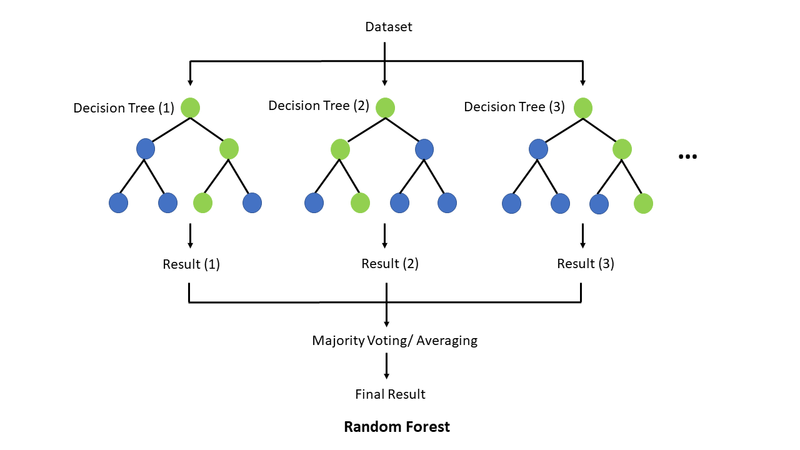
\includegraphics[width=\textwidth]{imagenes/random_forest_majority_vote.png}
	\caption{Voto por mayoría en el ``bosque''.}
	\label{fig:voto_mayoria}
\end{figure}

\subsection{LightGBM}
\label{subsubsec:eda_lgbm}

LightGBM (\textit{Light Gradient Boosting Machine}) es un framework de gradient boosting desarrollado por Microsoft en 2017 ~\parencite{2017lightgbm}. Este modelo optimiza el proceso de entrenamiento mediante innovaciones en la forma de construir los árboles y muestrear los datos. Mientras que Random Forest construye árboles de forma independiente y paralela, LightGBM los construye secuencialmente, donde cada nuevo árbol se especializa en corregir los errores de los anteriores.

\subsubsection*{Arquitectura y funcionamiento}

El proceso de $boosting$ funciona de la siguiente manera:

\begin{enumerate}
    \item Se entrena un primer árbol simple que intenta clasificar las instancias según las etiquetas.
    \item Se identifican las que este primer árbol clasificó incorrectamente.
    \item Se entrena un segundo árbol enfocado específicamente en esos casos difíciles.
    \item Se combinan ambos árboles para mejorar la precisión global.
    \item El proceso se repite construyendo decenas o cientos de árboles, cada uno corrigiendo los residuos de los anteriores.
\end{enumerate}

\subsubsection*{Innovaciones clave}

A continuación mostramos algunos aspectos por los cuales este modelo resulta interesante de aplicar al reconocimiento de voz clonada por IA:

\begin{itemize}
    \item \textbf{Crecimiento por hoja (\textit{leaf-wise})}: Los árboles crecen expandiendo la hoja que más puede reducir el error en cada paso, lo que produce árboles más profundos en las regiones problemáticas y más eficientes en las fáciles.
    
    \item \textbf{Muestreo basado en gradientes (\textit{GOSS, Gradient-based One-Side Sampling})}: Durante el entrenamiento, LightGBM identifica qué instancias tienen mayor error y las prioriza. Esto permite entrenar con datasets grandes sin procesar toda la información redundante.
    
    \item \textbf{Agrupación de características (\textit{EFB, Exclusive Feature Bundling})}: LightGBM agrupa las características que no suelen tomar valores iguales a 0 para reducir la dimensionalidad.
\end{itemize}

\subsubsection*{Proceso de clasificación}

Cuando una nueva instancia llega para ser clasificada:

\begin{itemize}
    \item Pasa secuencialmente por todos los árboles construidos.
    \item Cada árbol aporta una corrección o ajuste a la predicción anterior.
    \item La suma ponderada de todas las contribuciones produce la clasificación final (probabilidad de pertenecer a una clase).
\end{itemize}

\subsubsection*{Hiperparámetros}

Vamos a explicar los hiperparámetros más conocidos en los modelos LightGBM: 

\begin{itemize}
	\item \textbf{max depth}: Limita la profundidad máxima que pueden alcanzar los árboles durante el entrenamiento.

	\item \textbf{num leaves}: Determina el número máximo de hojas por árbol.
	
	\item \textbf{learning rate}: También conocido como $shrinkage rate$ o eta \(\eta\), este parámetro controla la velocidad a la que se actualizan los pesos del modelo después de cada iteración de $boosting$.
	
	\item \textbf{n estimators}: Determina el número máximo de iteraciones de $boosting$ que se realizarán, lo que equivale al número de árboles que se construirán.
	
	\item \textbf{reg alpha y reg lambda}: Estos parámetros aplican regularización L1 ($lasso$) y L2 ($ridge$) respectivamente para controlar la complejidad del modelo y prevenir el sobreajuste.
	
	\item \textbf{objective}: Define la tarea de aprendizaje que debe realizar el modelo y la función de pérdida que se optimizará durante el entrenamiento.
	
	\item \textbf{boosting type}: Determina el algoritmo específico que LightGBM utilizará para construir los árboles secuencialmente.
\end{itemize}

\subsubsection*{Ventajas específicas para detección de deepfakes}

Ahora veamos qué ventajas presenta LightGBM para detección de $deepfakes$:

\begin{itemize}
    \item \textbf{Alta precisión}: El enfoque secuencial de corrección de errores suele superar a Random Forest en problemas complejos como la detección de deepfakes.
    
    \item \textbf{Eficiencia computacional}: El muestreo inteligente permite entrenar con grandes volúmenes de audios en menos tiempo que otros métodos de $boosting$.
    
    \item \textbf{Manejo de desequilibrios}: Si existen desbalances entre clases, LightGBM incorpora mecanismos para ponderar las muestras adecuadamente.
    
    \item \textbf{Early stopping}: Se puede configurar para que detenga el entrenamiento cuando añadir más árboles no mejora la validación, evitando sobreajuste.
\end{itemize}

\subsection{Support Vector Machines (SVM)}
\label{subsubsec:eda_svm}

Las Máquinas de Vectores de Soporte (\textit{Support Vector Machines}, SVM) son un conjunto de algoritmos de aprendizaje supervisado desarrollados por Vladimir Vapnik y su equipo en AT\&T Bell Laboratories durante la década de 1990 ~\parencite{1995svm}. Originalmente diseñadas para clasificación binaria, las SVM se han convertido en uno de los métodos más robustos y teóricamente fundamentados del aprendizaje automático.

\subsubsection*{Fundamento y funcionamiento}

El objetivo fundamental de una SVM es encontrar un hiperplano que separe las clases (en nuestro caso dos, voces reales y voces generadas por IA) con el máximo margen posible. La clave de reside en que no cualquier línea divisoria es válida: el algoritmo busca aquella que maximiza la distancia entre la línea y los puntos más cercanos de cada clase. Estos puntos críticos, que ``sostienen'' el margen, reciben el nombre de \textbf{vectores de soporte} (\textit{support vectors}), de donde el algoritmo toma su nombre.

El proceso de entrenamiento de una SVM puede entenderse en los siguientes pasos:

\begin{enumerate}
    \item \textbf{Identificación de vectores de soporte}: El algoritmo examina todos los puntos de entrenamiento (instancias) e identifica aquellas que son más difíciles de clasificar, es decir, las que están más cerca de la frontera entre clases.
    
    \item \textbf{Maximización del margen}: A partir de estos vectores de soporte, la SVM calcula el hiperplano que maximiza la distancia a ambos lados. Este margen máximo proporciona la mejor capacidad de generalización: cuanto más ancho sea el margen, menor será la probabilidad de error al clasificar nuevas instancias.
    
    \item \textbf{Clasificación de nuevas muestras}: Una vez entrenado el modelo, para clasificar una nueva instancia, simplemente se calcula a qué lado del hiperplano se sitúa.
\end{enumerate}

\subsubsection*{El truco del kernel: Separando lo inseparable}

Uno de los mayores desafíos en la clasificación es que las instancias rara vez son linealmente separables en el espacio original de características. Es decir, no existe una línea recta (o hiperplano) que pueda separarlas perfectamente. Para abordar esta limitación, las SVM introducen el concepto de \textit{kernel} o núcleo.

El \textit{truco del kernel} funciona de la siguiente manera conceptual:

\begin{itemize}
    \item Los datos originales (no separables linealmente) se transforman implícitamente a un espacio de mayor dimensionalidad mediante una función matemática.
    \item En este nuevo espacio, es posible que los datos sí sean linealmente separables.
    \item La ventaja del kernel es que realiza esta transformación sin necesidad de calcular explícitamente las coordenadas en el espacio de alta dimensión, lo que sería computacionalmente costoso.
\end{itemize}

Los kernels más comúnmente utilizados son:

\begin{itemize}
    \item \textbf{Kernel lineal}: Asume que los datos son aproximadamente separables por un hiperplano. Útil cuando el número de características es muy grande.
    
    \item \textbf{Kernel polinomial}: Crea fronteras de decisión curvas mediante combinaciones polinómicas de las características originales.
    
    \item \textbf{Kernel RBF (\textit{Radial Basis Function})}: Es el más utilizado en muchos problemas. Proyecta los datos a un espacio de dimensionalidad infinita, permitiendo fronteras de decisión altamente complejas y no lineales. Se basa en la similitud entre muestras medida por distancia euclidiana:

    \[
    K(\mathbf{x}_i, \mathbf{x}_j) = \exp(-\gamma \|\mathbf{x}_i - \mathbf{x}_j\|^2)
    \]

    donde \(\gamma\) controla la influencia de cada muestra: un valor pequeño considera vecindarios amplios (frontera más suave), mientras que un valor grande se enfoca en vecindarios reducidos (frontera más ajustada a los datos).
\end{itemize}

\subsubsection*{Hiperparámetros}

Veamos cuáles son los hiperparámetros más influyentes en los SVM:

\begin{itemize}
    \item \textbf{C}: Controla el equilibrio entre tener un margen amplio y clasificar correctamente los puntos de entrenamiento.
    
    \item \textbf{kernel}: Es la función que transforma los datos a un espacio de mayor dimensión donde puedan ser separables linealmente.
    
    \item \textbf{gamma \(\gamma\)}: Específico de kernels no lineales (RBF, sigmoide o polinomial). Define cuánta influencia tiene un solo punto de entrenamiento.
    
    \item \textbf{probability}: Este parámetro $booleano$ determina si el modelo SVM debe calibrarse para proporcionar estimaciones de probabilidad junto con las predicciones de clase.
\end{itemize}

\subsubsection*{Ventajas específicas para detección de deepfakes}

Repasemos algunas de las ventajas que presentan los SVM para la detección de $deepfakes$:

\begin{itemize}
    \item \textbf{Fundamento teórico sólido}: A diferencia de otros métodos heurísticos, SVM está basada en la teoría de optimización convexa, lo que garantiza que la solución encontrada es óptima (máximo margen global).
    
    \item \textbf{Eficaz en espacios de alta dimensión}: Las características de audio pueden generar vectores de gran dimensionalidad (decenas o cientos de coeficientes). SVM maneja bien esta situación sin colapsar por la maldición de la dimensionalidad.
    
    \item \textbf{Robustez ante overfitting}: La maximización del margen proporciona una regularización natural que mejora la generalización, crucial cuando se trabaja con datasets limitados de voces $deepfake$.
    
    \item \textbf{Versatilidad mediante kernels}: La capacidad de elegir diferentes kernels permite adaptar el modelo a la estructura no lineal de los datos de audio sin necesidad de transformaciones manuales.
\end{itemize}

\subsection{Modelos de explicación}
Los modelos XAI (eXplainable Artificial Inteligence) han cobrado mucha importancia últimamente y más en términos de modelos de clasificación automáticos debido a la necesidad de saber el por qué se clasifican en un sitio u otro cada elemento, en nuestro caso cada audio.

\hspace{.7cm}
Dos modelos muy utilizados son el modelo SHAP (SHapley Additive exPlanations) y el modelo LIME (Local Interpretable Model-agnostic Explanations), que se utilizan para el análisis de audio sintético. SHAP, como ya sabemos, cuantifica la contribución de cada característica a la predicción final y ayuda a visualizar qué bandas de frecuencia son indicativas de manipulación. Viendo que a menudo revela distorsiones en las zonas de alta frecuencia que el detector suele utilizar para clasificar una muestra como "fake". Por otro lado, LIME, crea explicaciones locales perturbando la entrada y observando los cambios en la salida. También vimos que en forense de audio, LIME se utiliza para generar máscaras sobre espectrogramas, señalando los milisegundos específicos donde se detectan inconsistencias fónicas.

\hspace{.7cm}
Además de estos dos modelos, el modelo de Grad-CAM (Gradient-weighted Class Activation Mapping) se usa mucho junto con los modelos basados en CNN, ya que proporciona visualizaciones espaciales de las áreas del espectrograma que activan la decisión del modelo. Esto es importante para identificar si el modelo se está enfocando en anomalías espectrales o en ruido de fondo, por ejemplo.

\hspace{.7cm}
Por tanto, como hemos visto lo más utilizado y útil son técnicas independientes del modelo, como SHAP y LIME, que muestran que características han servido para que el modelo clasifique un audio como "real" o "fake", y complementariamente para modelos específicos de CNN que usan espectrogramas, se usa Grad-CAM, que muestra que zonas del espectrograma influyen más en la decisión del modelo.

\section{Metodología}

\subsection{Dataset}
Para encontrar un dataset público que tuviera voces tanto reales como clonadas y que ademas fueran por pares (i.e. un audio de voz real cuya transcripción es "Hoy he comido en un restaurante chino" y un audio clonando dicha voz diciendo lo mismo) ha sido complicado. Hemos echado un ojo a bastantes datasets. Vamos a comentar los que hemos descartado y por qué.

%En cuanto a la creación de nuestro propio dataset, lo primero es explicar las dos razones que nos llevaron a tomar esta decisión. La primera es por el tamaño del mismo; es más fácil hacer pruebas con un dataset más pequeño, y segundo porque así tenemos más controlados los audios que usamos para estas pruebas.

\begin{enumerate}
	\item HABLA \cite{3tamayoflorez23_interspeech}: Este dataset cuenta con una gran cantidad de audios tanto reales, como generados (con técnicas como TTS) y voces clonadas (con técnicas como Cycle-GAN). Lo hemos descartado principalmente por no contar con pares de audios, aunque tal vez podamos hacer pruebas con este dataset más adelante.
	\item audioMNIST \citep{4BECKER2024}: Este dataset cuenta con 30 mil audios de los números del 0 al 9 en inglés. Lo hemos descartado porque todos los audios son voces reales, por lo que no nos sirve para nuestra tarea.
	\item ASVSpoof2021 \citep{asvspoof2021_zenodo}: Este dataset forma parte de una serie de desafios internacionales organizados por la comunidad de verificación automática de audio cuyo objetivo es evaluar y mejorar los sistemas capaces de detectar voz manipulada. El dataset se compone de tres grupos de audio, todos ellos con voz real y generada mezclada, logical access con grabaciones transmitidas mediante canales de voz con efectos de codificación y transmisión, physical access con grabaciones de voz auténticas y ataques de reproducción en espacios físicos reales y speech deepfake con grabaciones generadas sintéticamente y comprimidas de formas distintas. Este dataset lo hemos descartado por no contar con pares de audio aunque se pueden rescatar algunos audios en inglés sobre todo para probar los modelos que probemos más adelante. % Poner cita
	\item Kaggle % (el que buscó rafa) poner cita y explicacion 
\end{enumerate}

\hspace{.7cm}
El dataset por el que nos hemos decantado se llama ODSS(https://www.ai4europe.eu/research/ai-catalog/odss-open-dataset-synthetic-speech). Hemos usado este conjunto de audios porque ya tiene creado un par para cada audio, lo que nos ahorra tiempo de generar nuestros propios audios. A esta ventaja, se le suma que ODSS ya contenía audios en Inglés y en Español, ambos idiomas son sumamente hablados por lo que es interesante centrarse en ellos.

\hspace{.7cm}
Con todo esto mencionado, hemos tomado un subset de 100 audios de cada idioma. La mitad son audios naturales y la otra mitad audios generados. Más adelante probaremos a usar más cantidad de audios y compararemos el rendimiento.


\subsection{Preprocesamiento} %Si se hace, añadirlo


\subsection{Extracción de características}
%\addvspace{2\parskip}
Para la transcripción de los audios usamos modelos de vosk(https://alphacephei.com/vosk/models). Esto se debe a que tiene modelos para ambos idiomas que vamos a usar y además, 2 modelos dentro de cada lenguaje. El que usamos para las pruebas es el small  ya que es más rápido y por lo tanto más útil para esta primera fase pero dejamos en consideración el modelo full para futuras fases ya que tiene mayor precisión. 
Sobre esto, cabe mencionar que primero probamos el modelo whisper pero tras varias pruebas con errores y la incapacidad para hacer funcionar, lo descartamos y es cuando escogimos vosk para esta tarea.

\subsection{Modelos de clasificación}


\subsection{Modelos de explicación}

\chapter{Conclusiones}

Tras terminar de revisar todo el proceso, desde la introducción del problema hasta las pruebas con modelos y una pequeña prueba real, se puede apreciar que el tema de esta investigación es para nada trivial, pues diferentes modelos tienen diferentes resultados. Se pueden ver claras diferencias entre los modelos específicos para la voz frente a los modelos generales (los que entrenan con datos tabulares). Los generales parecen tener cierta predisposición por algunas características, es decir, les otorgan una alta importancia frente al resto de características. Esto, si bien no es algo directamente negativo, si puede acarrear a malas predicciones, por ejemplo, si se modificasen dichas características ligeramente y los modelos cambiaran su predicción y, quizás, dichos cambios fuesen imperceptibles para el oído humano. En los modelos específicos hemos visto resultados más moderados, pero no por ello significa que sean peores que los otros modelos, SEGUIR DESARROLLANDO  

En la prueba real se han escogido 4 audios, dos en español y dos en inglés, de los cuales uno es real y el otro generado. Se ha podido ver, en forma de simulación en código, cómo sería el análisis de una voz nueva, su clasificación en real o generada, y el uso de métodos que explican la predicción de los modelos. En esta prueba se ha visto que es de vital importancia los audios con los que se entrenan los modelos, puesto que uno que llega para ser clasificado, de ser de distinta calidad (ruido de fondo, claridad de la voz, pausas, etc.), puede generar predicciones equivocadas, por lo que un buen dataset con diversidad de condiciones es necesario para un correcto funcionamiento de los modelos.

Se concluye con que este trabajo establece un buen punto inicial a la resolución de la detección de voces generadas y que los resultados aquí vistos muestran la viabilidad de esta.


ESTO ME PARECE MAS ESTILO RESUMEN
Como se ha mencionado, este proyecto se ha elaborado en el marco de la detección de voz sintética, es decir, voces suplantadas o \emph{deepfakes}. Durante la investigación del estado del arte para este problema a resolver se han encontrado modelos de aprendizaje automático tanto específicos para reconocimiento de voz como otros más generales, que entrenan en base a los datos tabulares de esta. En este punto también se exploraron diferentes métodos

\section{Trabajo futuro}

El trabajo desarrollado establece una base sólida para la detección de \textit{deepfakes} de audio mediante el uso de distintos métodos de IA y técnicas XAI.
Actualmente, el producto final del trabajo consiste en un pipeline que permite aplicar, sobre un audio de entrada, todos los modelos de clasificación y explicación estudiados en el capítulo~\ref{sec:metodologia}. Este pipeline genera como salida los resultados obtenidos por los distintos modelos de IA, combinados con gráficas resultantes de aplicar XAI sobre dichos resultados.

Aunque estas representaciones permiten observar qué factores han influido en la decisión de los modelos, su interpretación requiere de ciertos conocimientos técnicos y la explicación no siempre resulta suficientemente directa. Por ello, como trabajo futuro se propone el desarrollo de un explicador que actúe como una última capa entre los valores calculados por las técnicas XAI aplicadas en el pipeline y el resultado final mostrado.
La idea principal sería transformar el sistema actual, centrado en la visualización, en un enfoque basado en la interpretabilidad asistida. Es decir, el sistema no se limitaría a presentar gráficas, sino que también ofrecería explicaciones más fácilmente interpretables sobre la decisión final y sobre las evidencias que apoyan esta clasificación.

Asimismo, se sugieren dos tipos de explicadores que podrían resultar complementarios entre ellos. El primero estaría basado en \textbf{modelos grandes de lenguaje o LLM}. El objetivo de este primer explicador sería convertir salidas técnicas en explicaciones textuales más comprensibles y sintetizadas. Este enfoque presenta varias ventajas. En primer lugar, permitiría a usuarios no expertos comprender el motivo de la clasificación final. En segundo lugar, facilitaría la comparación entre los resultados de los distintos modelos.
En tercer lugar, permitiría generar informes automáticos que resuman las evidencias principales utilizadas para la clasificación del audio.

El segundo tipo de explicador propuesto estaría basado en \textbf{contrafactuales}. Mientras que las técnicas XAI responden principalmente a qué partes o características han influido en la decisión final, los contrafactuales responden a una pregunta diferente: ¿qué tendría que cambiar en el audio para que su clasificación fuera distinta?.
Este tipo de explicación es especialmente interesante porque también permite analizar la sensibilidad de los modelos ante modificaciones concretas de la entrada.

Este tipo de explicador podría indicar qué alteración mínima hace que los modelos cambien la clasificación original del audio. Según el tipo de modificación se contemplan tres posibilidades:
\begin{itemize}
    \item \textbf{Contrafactuales por segmentos temporales}: el sistema podría modificar, ocultar o sustituir segmentos determinados del audio y observar cómo cambian las predicciones.
    \item \textbf{Contrafactuales sobre espectrogramas}: este enfoque actuaría igual que el anterior pero realizando modificaciones sobre la representación espectral del audio.
    \item \textbf{Contrafactuales sobre características acústicas}: el explicador modificaría características acústicas como los MFCC o el pitch, con el objetivo de ver si se altera la salida de los modelos.
\end{itemize}

Sin embargo, esta propuesta contiene limitaciones que deben considerarse. En primer lugar, es necesario garantizar la fidelidad de las explicaciones respecto al comportamiento real de los modelos. En segundo lugar, se debe asegurar la trazabilidad, es decir, cada afirmación generada por el explicador se debe poder relacionar con una salida concreta del pipeline. En tercer lugar, los contrafactuales deben ser realistas y no consistir en modificaciones alejadas de la coherencia del dominio del audio.

En definitiva, el desarrollo de un módulo explicador mejoraría el alcance del sistema desarrollado, pasando de un pipeline capaz de detectar y mostrar evidencias en forma de gráficas a una herramienta capaz de justificar sus resultados de forma más clara e interpretable. Esta evolución contribuiría a mejorar la transparencia del proceso de clasificación, facilitaría el análisis de los audios y aumentaría la utilidad del sistema en contextos donde no solo se quiera conocer la clasificación de un audio, sino también comprender qué evidencias han llevado a tomar dicha decisión.

\section{Future Work}

The work developed establishes a solid foundation for the detection of audio deepfakes through the use of different AI methods and XAI techniques.
Currently, the final outcome of the work consists of a pipeline that makes it possible to apply, to an input audio, all the classification and explanation models studied in chapter~\ref{sec:metodologia}. This pipeline produces as output the results obtained by the different AI models, combined with graphs resulting from the application of XAI to those results.

Although these representations make it possible to observe which factors have influenced the models' decisions, their interpretation requires a certain level of technical knowledge, and the explanation is not always sufficiently direct. Therefore, as future work, the development of an explainer is proposed, acting as a final layer between the values computed by the XAI techniques applied in the pipeline and the final result shown.
The main idea would be to transform the current system, which is focused on visualization, into an approach based on assisted interpretability. That is, the system would not be limited to presenting graphs, but would also provide more easily interpretable explanations regarding the final decision and the evidence supporting this classification.

Furthermore, two types of explainers are suggested, which could be complementary to one another. The first would be based on \textbf{large language models, or LLMs}. The objective of this first explainer would be to convert technical outputs into more comprehensible and synthesized textual explanations. This approach presents several advantages. First, it would allow non-expert users to understand the reason behind the final classification. Second, it would facilitate comparison between the results of the different models.
Third, it would make it possible to generate automatic reports summarizing the main evidence used for the classification of the audio.

The second type of proposed explainer would be based on \textbf{counterfactuals}. Whereas XAI techniques mainly answer which parts or features have influenced the final decision, counterfactuals answer a different question: what would need to change in the audio for its classification to be different?
This type of explanation is especially interesting because it also makes it possible to analyze the sensitivity of the models to specific modifications of the input.

This type of explainer could indicate the minimum alteration that causes the models to change the original classification of the audio. Depending on the type of modification, three possibilities are considered:
\begin{itemize}
    \item \textbf{Counterfactuals based on temporal segments}: the system could modify, hide, or replace specific segments of the audio and observe how the predictions change.
    \item \textbf{Counterfactuals based on spectrograms}: this approach would operate in the same way as the previous one, but by performing modifications on the spectral representation of the audio.
    \item \textbf{Counterfactuals based on acoustic features}: the explainer would modify acoustic features such as MFCCs or pitch, with the aim of determining whether the models' outputs are altered.
\end{itemize}

However, this proposal contains limitations that must be considered. First, it is necessary to guarantee the fidelity of the explanations with respect to the actual behavior of the models. Second, traceability must be ensured; that is, each statement generated by the explainer must be linkable to a specific output of the pipeline. Third, counterfactuals must be realistic and must not consist of modifications that fall outside the coherence of the audio domain.

In conclusion, the development of an explainer module would improve the scope of the developed system, shifting from a pipeline capable of detecting and displaying evidence in the form of graphs to a tool capable of justifying its results in a clearer and more interpretable manner. This evolution would contribute to improving the transparency of the classification process, facilitate the analysis of audio recordings, and increase the usefulness of the system in contexts where the aim is not only to know the classification of an audio recording, but also to understand what evidence led to that decision.


\chapter{Pipeline}
\label{sec:pipeline}

Como cierre para el proyecto, se ha desarrollado un pipeline capaz de aplicar, al audio recibido como entrada, todos los modelos de IA y XAI explicados en el capítulo de \nameref{sec:metodologia}. Este pipeline tiene como objetivo reunir en un único ``notebook'' todos los modelos desarrollados a lo largo del proyecto. De este modo, permite facilitar la comparación de resultados y explicaciones entre modelos.

Cabe mencionar que el diseño de este pipeline constituye una de las aportaciones prácticas del proyecto, al integrar en una misma estructura modelos de distinta naturaleza y técnicas de explicabilidad complementarias. Esto permite analizar un mismo audio desde múltiples perspectivas, comparando no solo el resultado de clasificación, sino también la forma en que cada modelo justifica su decisión.

Con el fin de representar su estructura general, se ha diseñado un diagrama de flujo simplificado. Como se puede observar en la \autoref{fig:Arquitectura_pipeline}, los modelos se han dividido en dos grupos según el tipo de entrada que utilizan: por un lado, aquellos que operan sobre características extraídas del audio y, por otro, los que trabajan directamente con la forma de onda cruda. En cada grupo se indican tanto los modelos implementados como las técnicas de XAI aplicadas a cada uno de ellos.
\begin{figure}
    \centering
	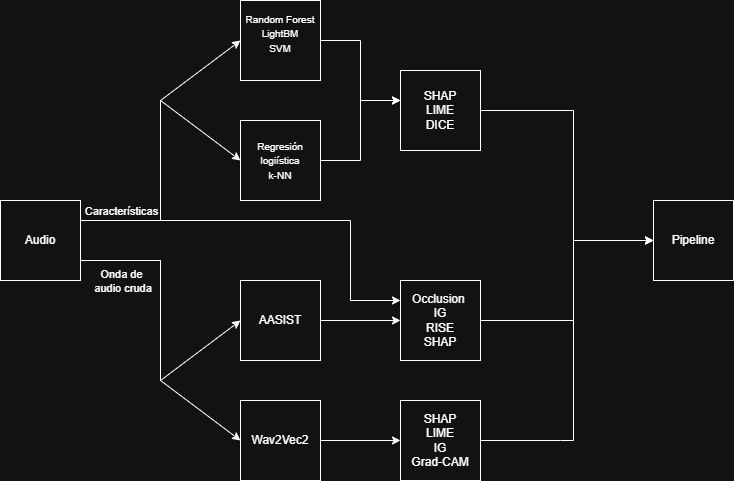
\includegraphics[width=\textwidth]{imagenes/Arquitectura_pipeline.png}
	\caption{Arquitectura del pipeline.}
    \label{fig:Arquitectura_pipeline}
\end{figure}

Para poder reutilizar los modelos entrenados durante el proyecto y evitar su reentrenamiento para cada caso, hemos empleado distintas técnicas para guardarlos. Los modelos que se entrenan con datos tabulares se han guardado mediante la librería joblib y su método \emph{to\_pkl()}, el cual guarda los pesos de los modelos y permite cargarlos fácilmente desde otro archivo. Sobre la forma de guardar el resto de modelos, se explicará en el apartado correspondiente a cada modelo.

La primera parte del ``notebook'' consta de una celda inicial con los imports necesarios, una segunda celda donde se especifica la ruta del audio que se quiere analizar y una tercera celda en la que se extraen las características del audio mediante la función ``\texttt{extract\_features}'' definida en el archivo funciones.py. A partir de ahí, cada modelo tiene su propia sección, en la que se muestra tanto la predicción como las explicaciones obtenidas con las técnicas de XAI asociadas a dicho modelo.

Además, el ``notebook'' está organizado en secciones correspondientes a cada modelo, lo que permite ejecutar cada uno de ellos de forma independiente.

\section{AASIST}

Para poder usar el modelo, lo primero ha sido guardarlo con la función torch.save(). Hemos usado esta función porque nos permite, no solo guardar el modelo para calcular la predicción final, sino también guardar la capa ``sinc-convolution'' para poder aplicar Integrated Gradients sobre ella. Para cargar el modelo, hemos usado la función torch.load() sobre el archivo guardado y la clase model del archivo AASIST.py de la carpeta Modelos/German.

Una vez cargado, se usan las funciones cargadas del archivo funciones\_AASIST.py que contiene todas las funciones necesarias para poder aplicar el modelo y las distintas técnicas de XAI. Primero, se ejecuta la función ``\texttt{score\_audio}'' que devuelve los resultados en forma de diccionario con cuatro claves: ``logits'', un tensor que contiene los ``logit'' para ambas clases; ``score\_bonafide'', el valor de ``logits'' para la clase ``bona fide''; ``prob\_bonafide'', la probabilidad de que el audio sea ``bona fide'' calculada a partir del ``logit'', y ``pred\_clase'', que muestra la clase predicha por el modelo.

A continuación, se ejecuta la función ``\texttt{aplicar\_XAI}'' que muestra las gráficas resultantes de aplicar las técnicas de XAI explicadas en \nameref{subsubsec:res_aasist}.

\section{Wav2Vec2}

Para poder reutilizar el modelo, es necesario guardar tanto el modelo entrenado como el extractor de características. Para ello, se utiliza el método \texttt{save\_model()} de la clase \texttt{Trainer}, junto con el método \texttt{save\_pretrained()} de \texttt{Wav2Vec2FeatureExtractor}. Ambas clases provienen de la librería \texttt{Transformers}.

Una vez guardados, con la función \texttt{from\_pretrained} de las clases \texttt{Wav2Vec2ForSequenceClassification} y \texttt{Wav2Vec2FeatureExtractor} puedes cargar tanto el modelo como el extractor de características.

Tras cargar lo que necesitamos, emplearemos la función \texttt{generar\_predicciones} del archivo \texttt{funciones\_wav2vec2} a la que pasándole el modelo, el extractor y el audio te devolverá tanto la salida del modelo (logits) como su predicción para ese audio (score).

Para generar las explicaciones de ese audio necesitamos usar los 200 audios de nuestro dataframe junto con su label. Con los audios usaremos la función \texttt{preprocesamiento} de \texttt{funciones\_wav2vec2} que nos devolverá los espectrogramas de todos los audios en forma de tensor de \texttt{torch} y agruparemos todos los labels en otro tensor.

Ahora que tenemos nuestro X\_train (tensor de los espectrogramas) y nuestro y\_train, podemos usar la función \texttt{build\_surrogate} y posteriormente la función \texttt{fit} de \texttt{torch} para entrenar nuestro surrogate model sobre el que aplicaremos las técnicas de XAI.

Por último, usaremos la función \texttt{mostrar\_graficas} de \texttt{funciones\_wav2vec2} que nos generará la gráfica del espectrograma del audio y las explicaciones del Shap, Integrated Gradients, Lime y Grad Cam.

Resultados: \ref{fig:Resultados_pipeline_wav2vec2}

\section{Random Forest}

Para empezar, vemos que el modelo, al predecir sobre los nuevos audios en español, los clasifica correctamente. Luego, para ver las explicaciones llamamos a las distintas funciones que habíamos definido. 

SHAP, tanto local como global, nos muestra que las importancias que otorga a los nuevos audios son similares (en valor y en orden) que los que vimos en \ref{res_xai_rf}, como vemos en \ref{fig:pipe_shap_rf_esp_1}, \ref{fig:pipe_shap_rf_esp_2} y \ref{fig:pipe_shap_rf_global}. También hemos probado a visualizar las explicaciones de los audios en inglés y, vemos que el modelo no parece tener \emph{transfer learning} entre idiomas (recordemos que los modelos tabulares se han entrenado con audios en español), ya que las importancias tienden a ser de menor valor y a ser siempre positivas. Esto lo podemos ver en \ref{fig:pipe_shap_rf_eng_1} y \ref{fig:pipe_shap_rf_eng_2}.

LIME nos muestra también que la característica más importante es ``spectral flatness'' y, además, mantiene unos umbrales de clasificación similares a los que vimos previamente (ver \ref{fig:pipe_lime_rf}).

DiCE nos da 3 instancias modificadas para que una instancia generada (audio generado que entra) sea clasificado como real, como vemos en \ref{tab:pipe_dice_rf}. Estas modificaciones son muy similares a las que vimos antes, centrándose principalmente en ``spectral flatness''.

\section{LightGBM}

En primer lugar, vemos que el modelo clasifica correctamente los nuevos audios. Ahora veamos los resultados de las funciones de explicación. 

SHAP, tanto local como global, nos muestra que las importancias son iguales que las que vimos en \ref{res_xai_lgbm}, es decir, clasifica únicamente basándose en ``spectral flatness'', como vemos en \ref{fig:pipe_shap_lgbm_esp_1}, \ref{fig:pipe_shap_lgbm_esp_2} y \ref{fig:pipe_shap_lgbm_global}. Podemos ver sobre los audios en ingles en \ref{fig:pipe_shap_lgbm_eng_1} y \ref{fig:pipe_shap_lgbm_eng_2}, aquí sigue tendiendo a clasificar como real y los valores de las importancias difieren de los audios en español.

LIME nos dice, como antes, que la característica más importante es ``spectral flatness'' con un dominio absoluto en la clasificación, como se aprecia en \ref{fig:pipe_lime_lgbm}.

DiCE nos da 3 instancias modificadas para que el nuevo audio generado sea clasificado como real, como vemos en \ref{tab:pipe_dice_lgbm}. Dichas modificaciones se centran en modificar el valor de ``spectral flatness''.

\section{Support Vector Machine}

Antes de ver la explicación de los nuevos audios con SVM, observamos que el modelo los clasifica correctamente.

En SHAP local vemos que las importancias cambian: en el audio generado tienen un peso mayor en ``spectral flatness'', mientras que en el audio real tienen un peso distribuido entre varias características, entre las que ``spectral flatness'' no aparece, como vemos en \ref{fig:pipe_shap_svm_esp_1} y \ref{fig:pipe_shap_svm_esp_2}. Por otro lado, en SHAP global podemos apreciar mejor que los audios clasificados como generados sí toman en cuenta dicha característica (con alto valor), mientras que los clasificados como reales tienen pesos más moderados, como aparece en \ref{fig:pipe_shap_svm_global}. Por último hemos probado a hacer, como antes, la explicación de los audios en inglés y podemos ver que tiene un rendimiento similar al de los modelos anteriores, es decir, pesos moderados y tendencia a clasificar como real. Esto lo encontramos en \ref{fig:pipe_shap_svm_eng_1} y \ref{fig:pipe_shap_svm_eng_2}.

LIME nos dice que la característica más importante, en el audio nuevo generado, es ``spectral flatness'' y, además, mantiene unos umbrales de clasificación similares a los que ya habíamos visto (ver \ref{fig:pipe_lime_svm}).

\section{Trabajo Individual}

\subsubsection{Iván Pastor Sacristán}

\begin{enumerate}
	\item Investigación del estado del arte: Investigué sobre el estado actual de la detección de deepfakes. Durante la investigación leí dos papers. En el primero hablaban sobre adaptación de los modelos a nuevos conjuntos de datos distintos de los que se usaron para entrenarlo y probarlo. En el segundo paper se centraban en un modelo capaz de clasificar correctamente los audios, aún y cuando los generados por IA habían sido modificados tanto en el dominio de la frecuencia como en el del tiempo para añadirles defectos característicos de los audios humanos como el ruido. %Añadir los enlaces a los papers en la bibliografía
	
	\item Prueba del dataset WaveFake: Hice una primera versión del extractor de características entre las que se incluyen rms, zcr, pitch, mfcc's, duración, transcripción, espectral centroid, espectral rolloff y el espectral bandwidth.
	
	\item Prueba del dataset ASVSpoof2021: Usé el mismo extractor de características e hice un clasificador difuso en el que, basándome en las características extraídas, clasifique los audios por género y edad aparente.
	
	\item Modelo compuesto: El modelo se basa en hacer un embedding de las características con un perceptrón multicapa (MLP), hacer un embedding del espectrograma del audio con una red neuronal convolucional (CNN), concatenarlos, y luego usar esos embeddings como entrada de un MLP + clasificador difuso que es lo que se encargará realmente de la tarea de clasificación.
	
	\item Fine-tuning Wav2Vev2: Usé el modelo desarrollado por Meta Wav2Vec2 y le hice un fine-tuning con nuestro dataset para que se enfocara en la clasificación de audios. Luego procesé la salida del modelo para pasar de la tupla que me devuelve el modelo a un valor entre 0 y 1 que indique la confianza de que un audio sea generado.
	
	\item XAI sobre Wav2Vec2: Sobre el modelo Wav2Vec2, no se puede aplicar directamente IA explicable ya que la entrada son embeddings, para ello lo que he hecho ha sido dividir entre las características y el espectrograma de Mel. Para las características usa Shap y Lime sobre surrogate models que imitan la salida de Wav2Vec2 y para los espectrogramas de Mel use una CNN a la que le apliqué Shap, Lime, Integrated gradients y Grad Cam.



\begin{contribucion}{Jorge Aured Zarzoso}

\begin{itemize}

	\item Investigué sobre las motivaciones para investigar sobre la detección de voz generada por IA con dos papers. En estos se hablaba de cómo las personas hemos perdido la capacidad de detectar correctamente cuando un audio es real o no. Es importante ver que este es un problema que ha ganado popularidad en los úlitmos años de la mano de los avances de los modelos de inteligencia artificial. También investigué sobre las técnicas de clonación de voz para su análisis en relación con las ciencias forenses, donde es vital identificar a las diferentes personas en un caso.
	
	\item Investigué sobre qué características son relevantes en la voz y cómo extraerlas mediante código. Esto ya que es crucial saber qué representa cada característica para tener una noción de qué puede tener en cuenta los modelos a la hora de predecir si un audio es real o no.  Apliqué las funciones que extraen las distintas características y creé un pipeline completo de extracción, así como una función a las que se le pasan n audios y devuelve las características de cada uno.
	
	\item Investigué parcialmente sobre la extracción de gráficas de la voz, para su uso en redes convolucionales (CNN).	
	
	 \item Sobre XAI investigué un enfoque de interpretabilidad dual (visual y auditiva), usando espectrogramas y reconstrucción de audio a partir de los scores de atribución. Se analiza cómo diferentes arquitecturas (CNN vs CNN-LSTM) y métodos XAI (LRP, Deep Taylor, Integrated Gradients) afectan la localización de formantes y la varianza rítmica, permitiendo una explicación al nivel de percepción humana.
	 
	 \item Investigué sobre el estado del arte de modelos que entrenan con datos tabulares. En concreto revisé los modelos LightGBM, Random Forest basados en árboles de decisión y SVM basado en separación óptima mediante hiperplano, para clasificación, leyendo varios papers y páginas oficiales. En dicha investigación profundicé en el funcionamiento de los modelos, viendo qué hiperparámetros tiene cada uno y para qué sirven, y qué ventajas tienen para la clasificación de audios en reales o generados.
	 
	 \item Investigué sobre datasets que nos pudieran servir para la investigación. Encontré audioMNIST y HABLA, el primero de los números del 0 al 9 y el segundo son voces en español de hispanoamérica. audioMNIST solo cuenta con voces reales, mientras que HABLA tiene tanto clonaciones de voz como ataques (hacer que una voz se parezca a otra). El primero lo descartamos por tener solo voces reales, y el segundo lo descartamos por solo tener audios en español.
	 
	 \item Para cada uno de los tres modelos he hecho un pipeline completo con tres partes claras: (1) un modelo baseline (dos en el caso de SVM debido al tipo de kernel) donde establezco a mano los hiperparámetros y lo entreno para ver sus resultados; (2) una validación cruzada para entrenar el modelo baseline con varios conjuntos de entrenamiento-validación y comprobar su estabilidad y overfitting; (3) una búsqueda de los hiperparámetros óptimos de cada modelo mediante un grid search; y (4) entrenar un modelo con dichos hiperparámetros óptimos y revisar su rendimiento. Por último, guardé cada modelo como archivo .pkl para poder usarlos en otros archivos.
	 
	 \item He hecho un pipeline completo para cada uno de los tres modelos, entrenándolos de varias formas para ver cuál funcionaba mejor. Este pipeline consta de un modelo baseline, una fase de cross validation y un grid search optimizando los parámetros. En cada paso visualicé los resultados de los modelos viendo su rendimiento. Al final del pipeline guardé como archivo .pkl los mejores modelos
	 
	\item He creado diversas funciones para generar explicaciones de los modelos, en concreto he hecho una función para SHAP (local y global), otra para LIME y otra para DiCE, y una cuarta para poder extraer características, reentrenar, y poder generar la explicación con una de las tres funciones anteriores. Además, esta última función permite reevaluar las métricas del modelo para ver su rendimiento tras eliminar algunas características. Con esto Apliqué las funciones a los tres modelos, haciendo pruebas según los resultados. 
	
	\item He aplicado los tres modelos en una prueba donde simulamos una aplicación real donde entran audios nuevos y debemos clasificarlos y generar las explicaciones. He cargado los modelos .pkl (ya entrenados) y he reutilizado las funciones de explicación que cree anteriormente, salvo la de extraer características.
	
	\item He redactado las partes de la memoria asociadas a mis modelos: estado del arte, experimentos y resultados.
	
	\item He escrito la sección de extracción de características, la de métricas de evaluación de los modelos, y la de proceso común de experimentación. También he escrito parcialmente la sección del dataset, la introducción, el resumen, y las conclusiones finales del proyecto.

\end{itemize}
\end{contribucion}

\newpage
\subsubsection{Germán Bravo Quintián}

\begin{itemize}
    \item En cuanto a mi investigación inicial sobre la detección de voz generada por IA, leí tres papers.
    \begin{enumerate}
        \item Paper sobre AASIST:  la motivación principal para desarrollar el modelo es porque algunos ataques de spoofing dejan huellas espectrales, otros temporales; y los modelos generalmente no miran ambos tipos.
        \item Paper sobre RawNEt2: aunque Rawnet2 fue diseñado originalmente para la verificación del hablante, en el paper proponen una adaptación de este modelo para el ámbito de la detección de spoofing. La motivación es crear un modelo que trabaje directamente sobre la onda cruda de audio para que pueda aprender características generales, reduciendo su dependencia sobre artefactos ya conocidos.
        \item Paper sobre ASVspoof2021: sobre la tarea Logical Access(LA), el paper introduce este dataset como mejora de los anteriores añadiendo mejoras como condiciones de transmisión, codificación y comprensión.
    \end{enumerate}
    \item Además, del dataset del último paper, investigue otros dos datasets que nos sirvieran para entrenar nuestros modelos. El primero, es “In-the-wild”, dataset en inglés, con audios reales y falsos que incluye voces de 58 personas famosas. El segundo es odss(Open Dataset of Synthetic Speech), que incluye 158 voces en inglés, alemán y español en el que cada audio falso tiene su correspondiente versión real.
    \item Creación de nuestro propio dataset de prueba teniendo en cuenta los datasets investigados por mis compañeros y los recién mencionados.
    \item Investigué sobre transcriptores de audio, intentando implementar el paquete de python de Whisper pero debido a dificultades en la tarea lo descarté. Finalmente, implementé “vosk”, creando una función que usando su modelo devolviera la transcripción.
    \item Paper de AASIST2: se centra en intentar solventar el problema de que al modelo le cuestan los audios cortos, esto se debe porque al haber menos información, hay menos nodos y menos relaciones por tanto. Cambios princiaples: usan Res2Net blocks, DCS y ALMFT.
    \item Paper de AASIST3:  cambios principales: redes Kolmogorov-Arnold, permiten modelar funciones complejas multivariadas; características de aprendizaje supervisado; más bloques residuales y técnicas de regularización.
    \item Paper de AASIST con "Speaker-Aware": da contexto sobre el peligro de la suplantación de voz, los distintos tipos de ataques y habla de los datasets de ASVspoof.
    \item ASVspoof 2019: A large-scale public database of synthesized, converted and replayed speech: ofrece contexto sobre el peligro de la suplantación de voz, los distintos tipos de ataques y habla de los datasets de ASVspoof.
    \item Paper sobre Integrated Gradients: explican los axiomas en lo que se basa, presentados como fundamentales para cualquier XAI; definen los fundamentos matématicas de la técnica y ofrece pruebas de IG sobre varias aplicaciones.
    \item Paper sobre Occlusion: el apartado 4.2 introduce el concepto de occlusion, aunque lo use para imágenes, lo usé como base para aplicarlo a AASIST..
    \item Paper sobre RISE: propone RISE como un modelo que solo necesita acceder a la entrada y a la salida sin tener en cuenta gradientes, pesos internos... Como para Occlusion, en el paper, se aplcia solo a imaágenes y he reconvertido la idea.
    \item En relación al uso de modelos, he creado todo el código para el uso de AASIST, además, de realizar todas las pruebas mencionadas en su apartado de metedologías. También, he desarrollado el código relacionado con su explicabilidad, es decir, la implementación de RISE, Integrated Gradients, Occlusion y el mostrado de ciertos niveles internos de la arquitectura. Por último, realicé el intento fallido de aplicar SHAP a un surrogate que imite a AASIST para intendar dar explicaciones a nivel de características.
    \item De la parte común de memoria, del estado del arte,he realizado la introducción y conclusión y he reescrito el apartado de Modelos de explicación.
    \item Sobre la parte de memoria sobre el modelo que he implementado, AASIST, he escrito todo lo relacionado, es decir, explicación en estado del arte, y implementación y explicación de resultados en metodología.
\end{itemize}

\begin{contribucion}{Rafael López Rodríguez}

\begin{itemize}

	\item Investigué sobre las motivaciones sociales y técnicas detrás de la creación de deepfakes, así como los problemas críticos que presenta la detección de audio clonado en la actualidad.
	
	\item Investigué sobre el estado del arte de los modelos de clasificación Regresión Logística y K-Nearest Neighbors (k-NN), profundizando en sus fundamentos matemáticos, sus hiperparámetros y su idoneidad para el manejo de características acústicas.
	
	\item Investigué exhaustiva sobre las técnicas de IA Explicable (XAI), analizando cuáles de ellas son aplicables específicamente al dominio del audio y la detección de fraude. Esto incluyó tanto técnicas post-hoc (que explican modelos ya entrenados) como técnicas ante-hoc (modelos interpretables por diseño).
	
	\item Estudié la viabilidad de aplicar arquitecturas intrínsecamente explicables como ProtoPNet y SincNet para la detección de audio, realizando pruebas para determinar si estas técnicas de explicabilidad ante-hoc aportarían valor frente a los métodos tradicionales.
	
	\item Desarrollé el código necesario para la implementación de los algoritmos de Regresión Logística y k-NN. Diseñé un flujo de trabajo que incluyó el ajuste fino de hiperparámetros y un análisis detallado de las métricas de rendimiento para optimizar la capacidad de detección.
	
	\item Apliqué técnicas de explicabilidad post-hoc a los modelos desarrollados, implementando SHAP (global y local), LIME (local) y DiCE (generación de explicaciones contrafactuales) para interpretar las decisiones del sistema.
	
	\item Redacté los apartados de Objetivos y Planificación dentro de la Introducción del proyecto.
	
	\item Redacté, en el bloque de Estado del Arte, las secciones correspondientes a los modelos de clasificación (Regresión Logística y k-NN) y a la totalidad de las técnicas de explicabilidad analizadas (SHAP, LIME, DiCE, Integrated Gradients, Grad-CAM, SincNet y ProtoPNet).
	
	\item Elaboré los apartados técnicos de la Metodología relativos a la implementación y el análisis de resultados de los modelos de Regresión Logística y k-NN.

\end{itemize}
\end{contribucion}


\backmatter

% Esto carga el archivo .bib. El nombre del archivo es "bibliografia.bib"
\printbibliography[heading=bibintoc]

\newpage
\subsection{Anexo}
\begin{figure}[H]
    \centering
	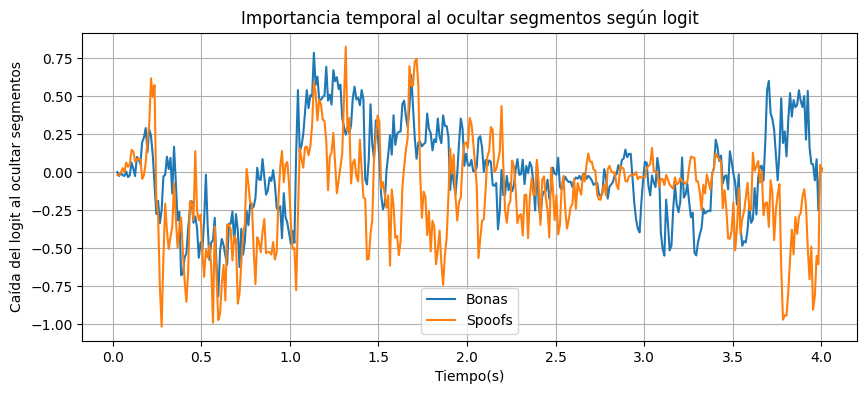
\includegraphics[width=\textwidth]{imagenes/AASIST_global_occlusion_temp_logit.png}
	\caption{Resultados de ``logit'' de la ocultación temporal en AASIST.}
    \label{fig:AASIST_global_occlusion_temporal_logit}
\end{figure}

\begin{figure}[H]
    \centering
	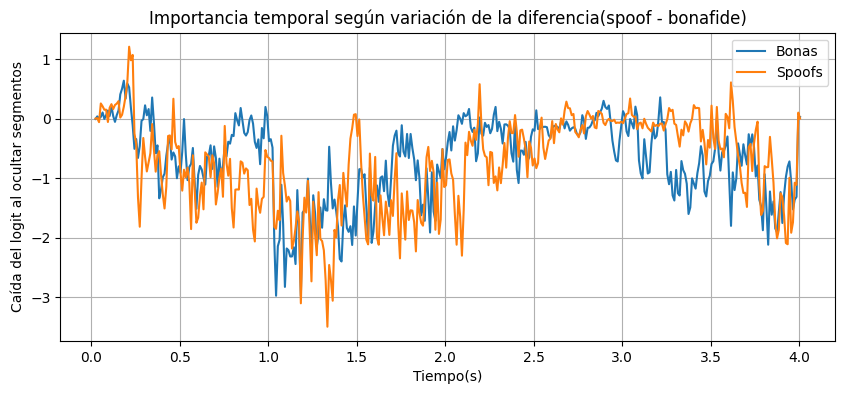
\includegraphics[width=\textwidth]{imagenes/AASIST_global_occlusion_temp_margin.png}
	\caption{Resultados de margen de la ocultación temporal en AASIST.}
    \label{fig:AASIST_global_occlusion_temporal_margin}
\end{figure}

\begin{figure}[H]
    \centering
	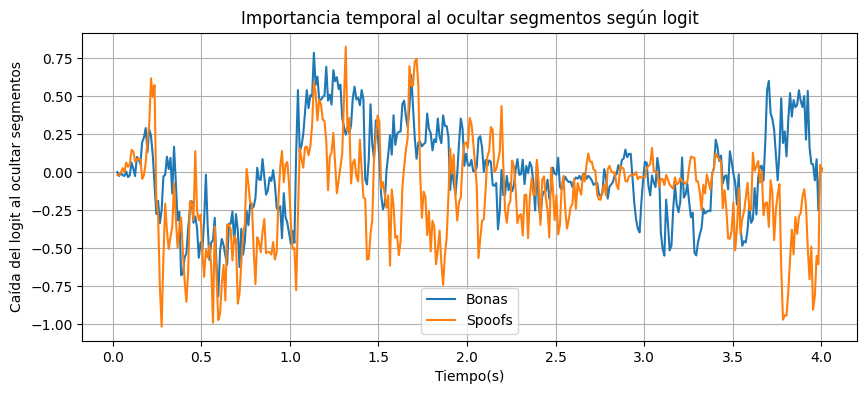
\includegraphics[width=\textwidth]{imagenes/AASIST_global_occlusion_frec_logit.png}
	\caption{Resultados de ``logit'' de la ocultación frecuencial en AASIST.}
    \label{fig:AASIST_global_occlusion_frecuencial_logit}
\end{figure}

\begin{figure}[H]
    \centering
	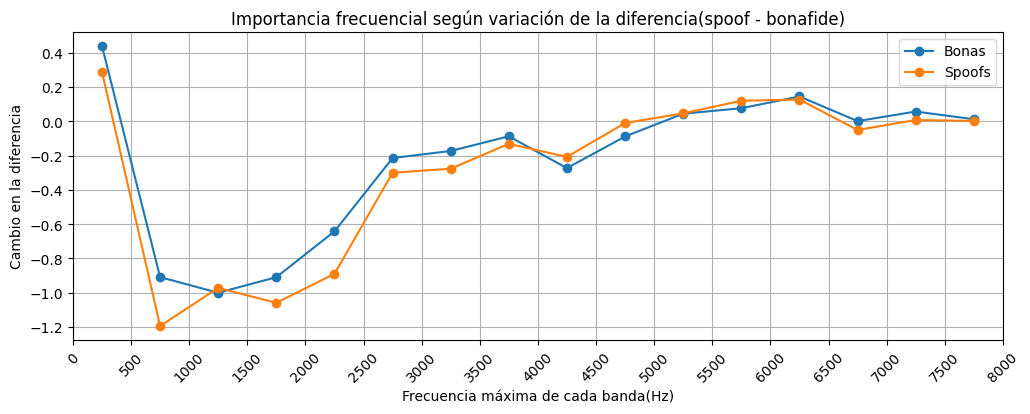
\includegraphics[width=\textwidth]{imagenes/AASIST_global_occlusion_frec_margin.png}
	\caption{Resultados de margen de la ocultación frecuencial en AASIST.}
    \label{fig:AASIST_global_occlusion_frecuencial_margin}
\end{figure}

\begin{figure}[H]
    \centering
    \begin{subfigure}[t]{0.49\textwidth}
        \centering
        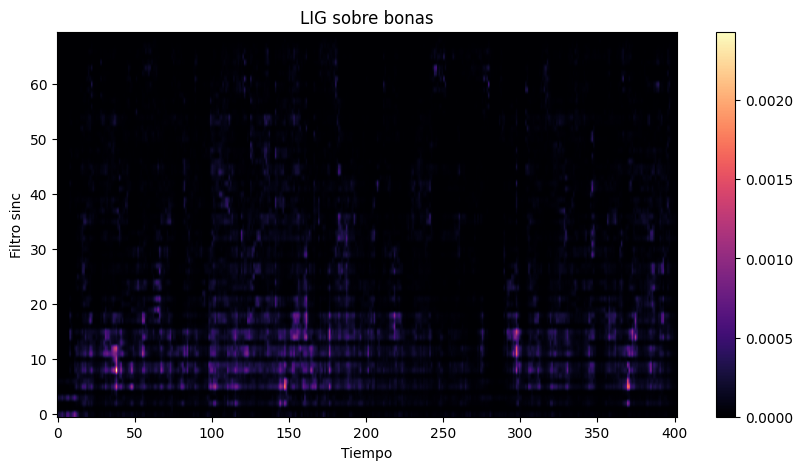
\includegraphics[width=\linewidth]{imagenes/AASIST_global_LIG_bonas.png}
        \caption{Mapa filtro-tiempo generado con IG para ``bonas''.}
        \end{subfigure}
    \hfill
    \begin{subfigure}[t]{0.49\textwidth}
        \centering
        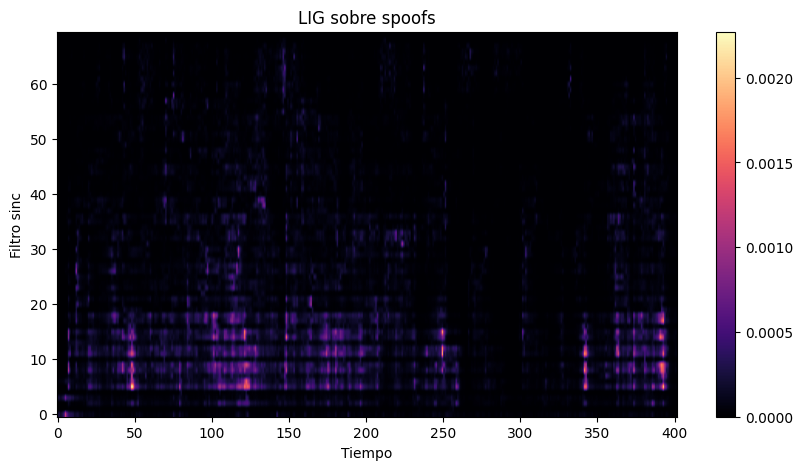
\includegraphics[width=\linewidth]{imagenes/AASIST_global_LIG_spoofs.png}
        \caption{Mapa filtro-tiempo generado con IG para ``spoofs''.}
    \end{subfigure}
    \caption{Mapas filtro-tiempo de la capa sinc-convolution generados con IG.}
    \label{fig:AASIST_global_LIG_mapas}
\end{figure}

\begin{figure}[H]
    \centering
    \begin{subfigure}[t]{0.49\textwidth}
        \centering
        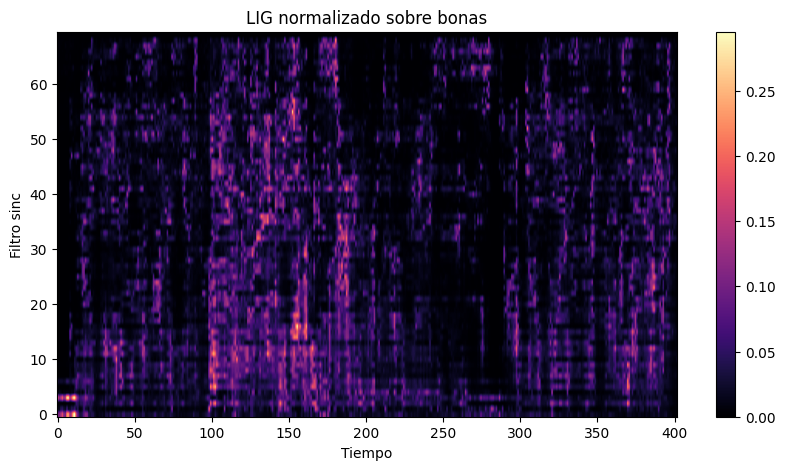
\includegraphics[width=\linewidth]{imagenes/AASIST_global_LIG_bonas_norm.png}
        \caption{Mapa filtro-tiempo normalizado generado con IG para ``bonas''.}
        \end{subfigure}
    \hfill
    \begin{subfigure}[t]{0.49\textwidth}
        \centering
        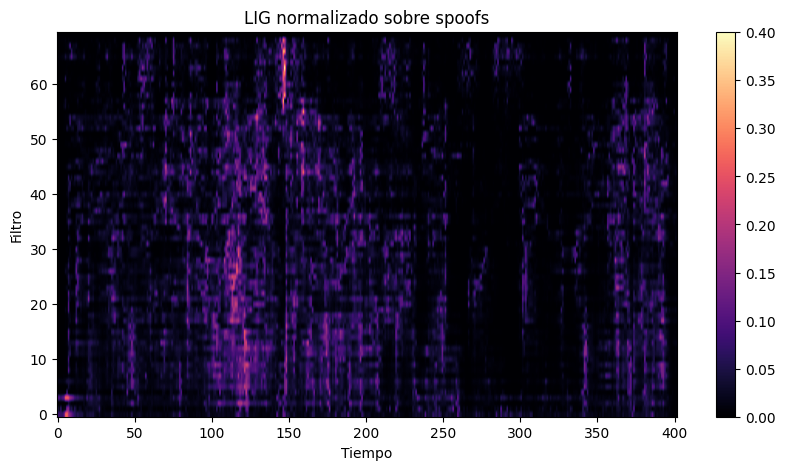
\includegraphics[width=\linewidth]{imagenes/AASIST_global_LIG_spoofs_norm.png}
        \caption{Mapa filtro-tiempo normalizado generado con IG para ``spoofs''.}
    \end{subfigure}
    \caption{Mapas filtro-tiempo de la capa sinc-convolution generados con IG normalizados.}
    \label{fig:AASIST_global_LIG_mapas_norm}
\end{figure}

\begin{figure}[H]
    \centering
	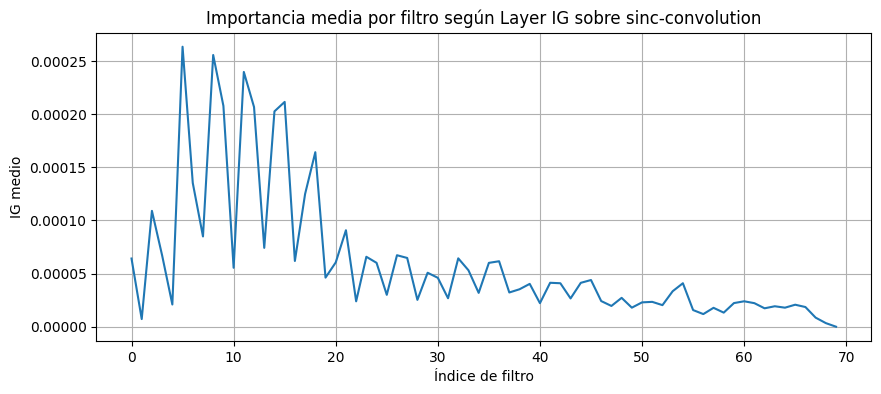
\includegraphics[width=\textwidth]{imagenes/AASIST_global_LIG_grafica.png}
	\caption{Gráfica filtro-tiempo de la capa sinc-convolution.}
    \label{fig:AASIST_global_LIG_grafica}
\end{figure}

\begin{figure}[H]
    \centering
	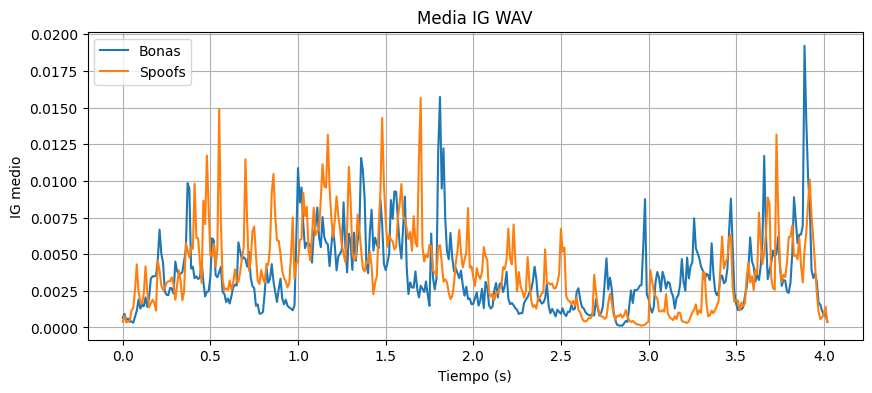
\includegraphics[width=\textwidth]{imagenes/AASIST_global_IG_audio.png}
	\caption{Importancia temporal al aplicar IG sobre onda de audio cruda.}
    \label{fig:AASIST_global_IG_audio}
\end{figure}

\begin{figure}[H]
    \centering
    \begin{subfigure}[t]{0.49\textwidth}
        \centering
        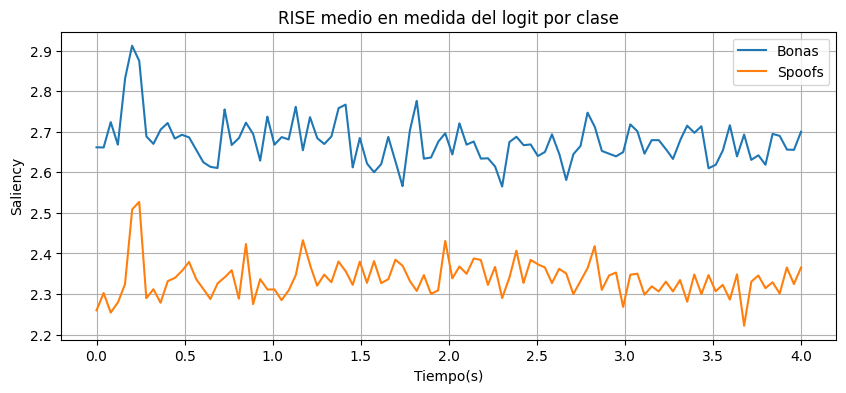
\includegraphics[width=\linewidth]{imagenes/AASIST_global_RISE_logit.png}
         \caption{Resultados de ``logit'' usando RISE.}
        \end{subfigure}
    \hfill
    \begin{subfigure}[t]{0.49\textwidth}
        \centering
        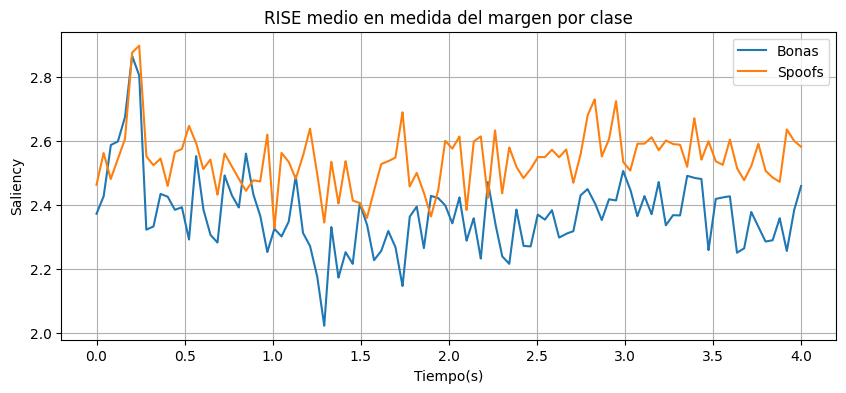
\includegraphics[width=\linewidth]{imagenes/AASIST_global_RISE_margen.png}
        \caption{Resultados de ``margin'' usando RISE.}
    \end{subfigure}
    \caption{Resultados de RISE.}
    \label{fig:AASIST_global_RISE}
\end{figure}

\begin{figure}[H]
    \centering
    \begin{subfigure}[t]{0.49\textwidth}
        \centering
        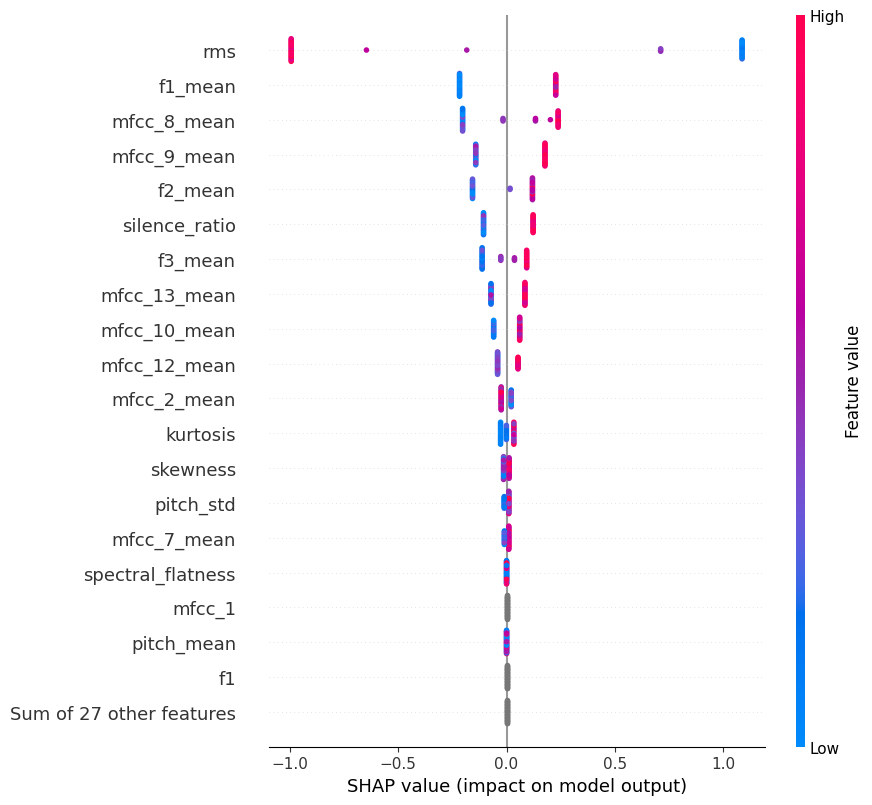
\includegraphics[width=\linewidth]{imagenes/AASIST_global_SHAP_clas.png}
        \caption{Agrupación de las gráficas SHAP del clasificador.}
        \end{subfigure}
    \hfill
    \begin{subfigure}[t]{0.49\textwidth}
        \centering
        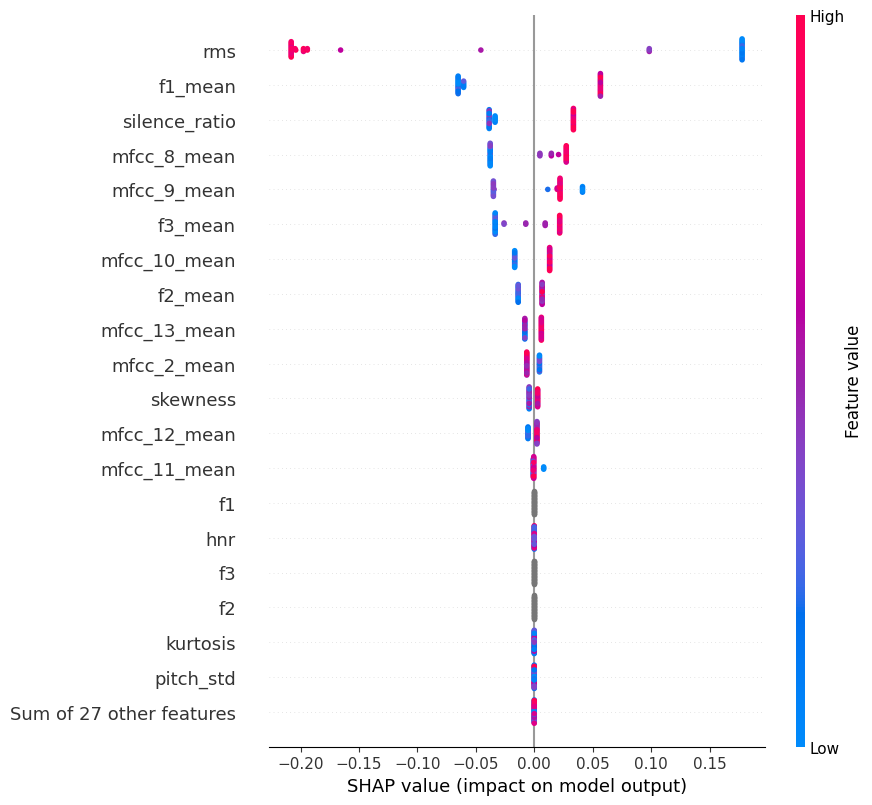
\includegraphics[width=\linewidth]{imagenes/AASIST_global_SHAP_reg.png}
        \caption{Agrupación de las gráficas SHAP del regresor.}
    \end{subfigure}
    \caption{Gráficas de importancia global de SHAP para el clasificador y el regresor.}
    \label{fig:AASIST_global_SHAP}
\end{figure}







\end{document}
